% Este archivo es parte de la memoria de libWiiEsp, protegida bajo la 
% licencia GFDL. Puede encontrar una copia de la licencia en el archivo fdl-1.3.tex

% Fuente tomada de la plantilla LaTeX para la realización de Proyectos Final 
% de Carrera de Pablo Recio Quijano.

% Copyright (C) 2009 Pablo Recio Quijano
% Copyright (C) 2011 Ezequiel Vázquez de la Calle

% -*-referencia.tex-*-

En este apéndice se incluye el manual de referencia completo de la biblioteca. Este manual aporta una visión en profundidad sobre todos los métodos, atributos y estructuras que componen la herramienta, y está generado con la herramienta Doxygen \cite{website:doxygen}.\\

Por otro lado, cada una de las clases documentadas en este manual viene acompañada por una exhaustiva explicación sobre su funcionamiento interno, así como ejemplos sencillos que ilustran cómo se debe emplear cada módulo a la hora de darle uso dentro de un videojuego desarrollado con \programa{LibWiiEsp}.\\

Nótese que, aunque se respetan los números de página dentro de este documento, la numeración de este apéndice difiere de la empleada durante el resto del escrito, debido a que este manual de referencia se ha importado directamente desde el archivo PDF generado con Doxygen.

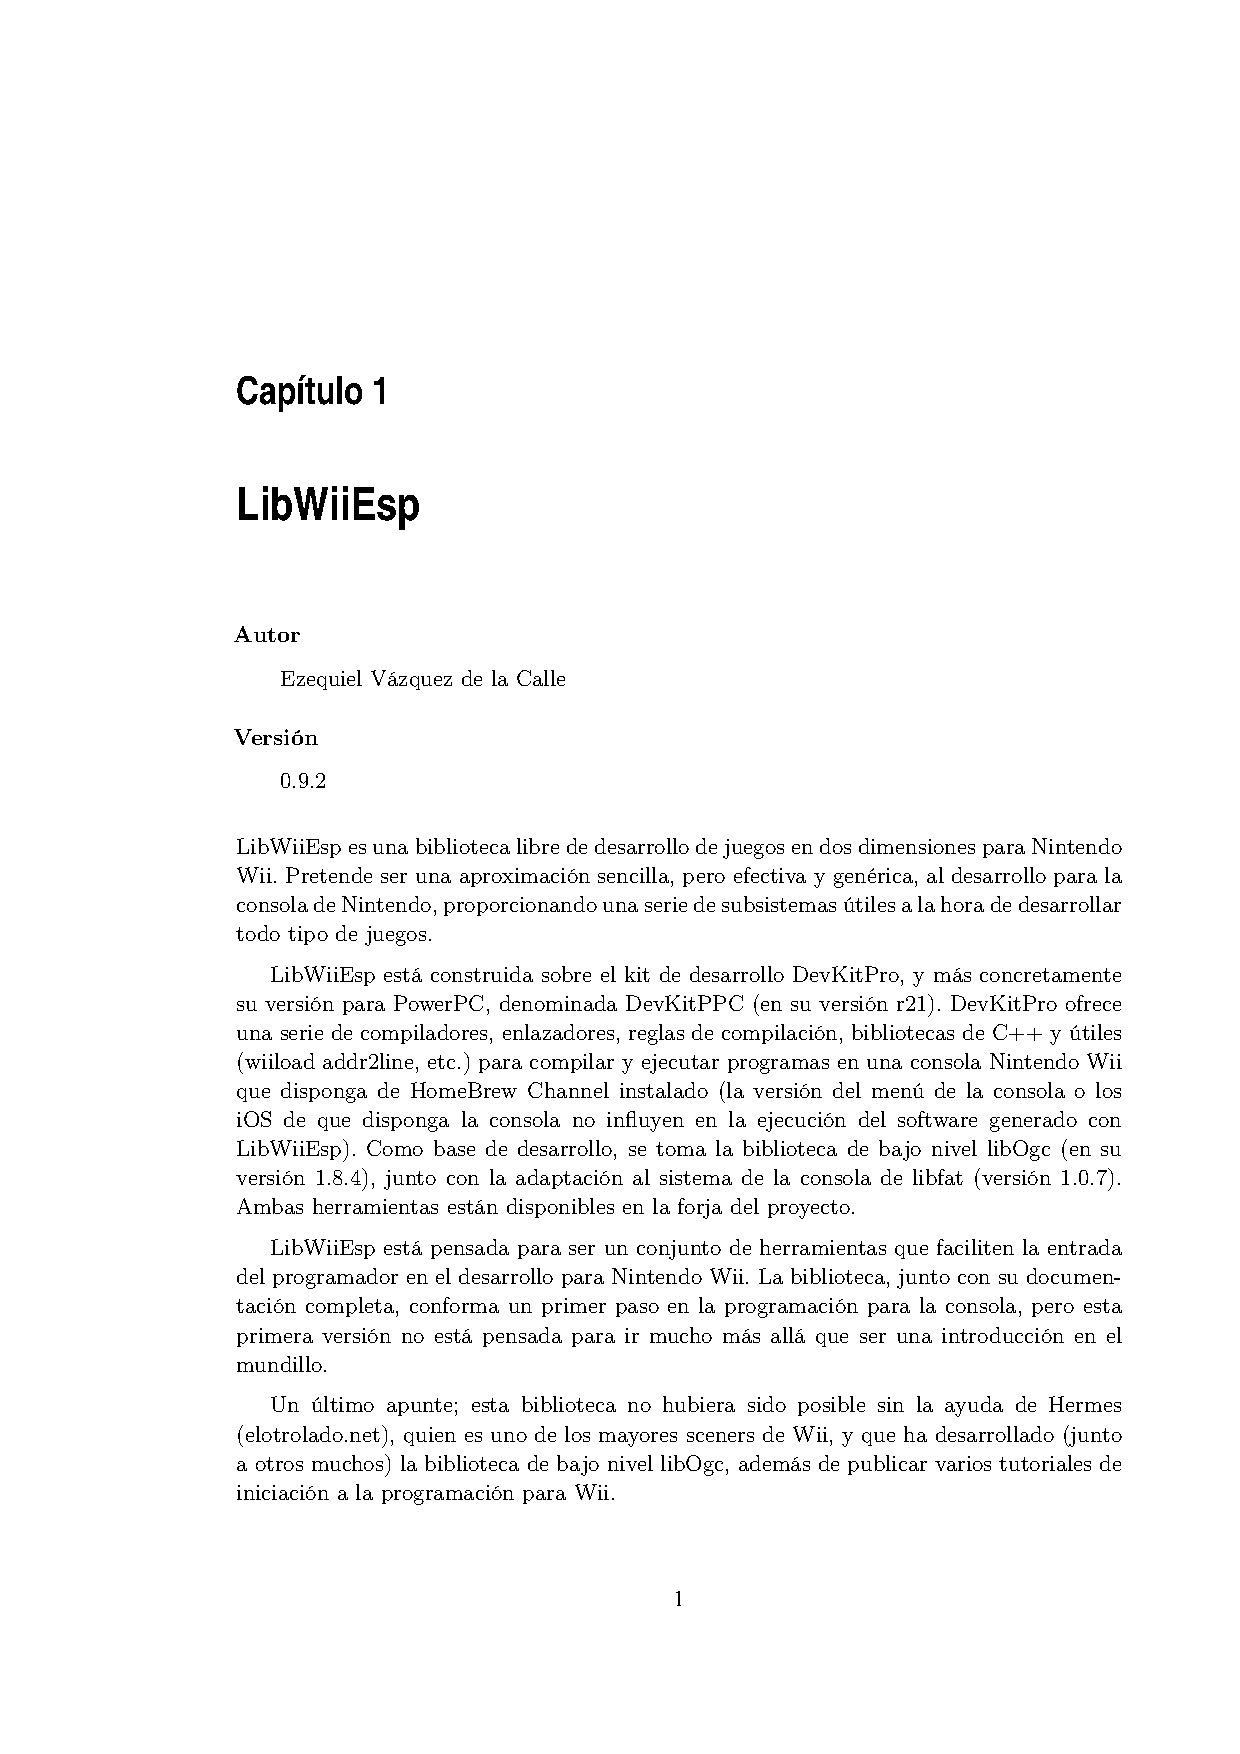
\includepdf[pages=-,pagecommand=\thispagestyle{fancy}]{./referencia/refman}
